\chapter{Applicazioni Lineari}
\label{ch:applicazioni-lineari}

Le applicazioni lineari sono le funzioni che ``rispettano'' la struttura di spazio vettoriale. Esse costituiscono il collegamento naturale tra la teoria astratta degli spazi vettoriali e il calcolo matriciale.

\section{Definizione e proprietà}
\label{sec:appl-lin-def}

\begin{definitionbox}[Applicazione lineare]
Siano $V$ e $W$ spazi vettoriali su $\mathbb{R}$. Una funzione $T \colon V \to W$ è un'\textbf{applicazione lineare} (o \textbf{omomorfismo}) se per ogni $\mathbf{u}, \mathbf{v} \in V$ e $\lambda \in \mathbb{R}$:
\begin{enumerate}
    \item $T(\mathbf{u} + \mathbf{v}) = T(\mathbf{u}) + T(\mathbf{v})$ \hfill (additività)
    \item $T(\lambda \mathbf{v}) = \lambda \, T(\mathbf{v})$ \hfill (omogeneità)
\end{enumerate}
Equivalentemente, $T(\lambda\mathbf{u} + \mu\mathbf{v}) = \lambda T(\mathbf{u}) + \mu T(\mathbf{v})$ per ogni $\lambda, \mu \in \mathbb{R}$.
\end{definitionbox}

\begin{examplebox}[Esempi di applicazioni lineari]
\begin{enumerate}
    \item La funzione $T \colon \mathbb{R}^3 \to \mathbb{R}^2$ definita da $T(x, y, z) = (x + y, \, 2z)$ è lineare.
    \item La proiezione $\pi \colon \mathbb{R}^3 \to \mathbb{R}^2$, $\pi(x,y,z) = (x,y)$ è lineare.
    \item La derivata $D \colon \mathbb{R}[x]_{\leq n} \to \mathbb{R}[x]_{\leq n-1}$, $D(p) = p'$ è lineare.
    \item La funzione $f(x) = x + 1$ da $\mathbb{R}$ in $\mathbb{R}$ \textbf{non} è lineare ($f(0) = 1 \neq 0$).
\end{enumerate}
\end{examplebox}

\begin{figure}[htbp]
  \centering
  
\includegraphics[width=0.6\textwidth]{ch04-linear-transformations}
  \caption{Quattro trasformazioni lineari fondamentali nel piano: rotazione, riflessione, scalatura e shear. Ciascuna mostra l'effetto sulla griglia unitaria.}
  \label{fig:ch04-linear-transformations}
\end{figure}

\begin{notebox}[Conseguenza immediata]
Ogni applicazione lineare manda il vettore nullo nel vettore nullo: $T(\mathbf{0}_V) = \mathbf{0}_W$. Se $T(\mathbf{0}) \neq \mathbf{0}$, la funzione non è lineare.
\end{notebox}

\begin{definitionbox}[Terminologia]
Un'applicazione lineare $T \colon V \to W$ si dice:
\begin{itemize}
    \item \textbf{Endomorfismo} se $V = W$.
    \item \textbf{Isomorfismo} se è biiettiva (iniettiva e suriettiva).
    \item \textbf{Automorfismo} se è un endomorfismo biiettivo.
\end{itemize}
\end{definitionbox}

\section{Nucleo e immagine}
\label{sec:nucleo-immagine}

\begin{definitionbox}[Nucleo e immagine]
Data $T \colon V \to W$ lineare:
\begin{itemize}
    \item Il \textbf{nucleo} (o \textbf{kernel}) è $\ker(T) = \{\mathbf{v} \in V : T(\mathbf{v}) = \mathbf{0}\} \subseteq V$.
    \item L'\textbf{immagine} è $\text{Im}(T) = \{T(\mathbf{v}) : \mathbf{v} \in V\} \subseteq W$.
\end{itemize}
\end{definitionbox}

\begin{theorembox}[Nucleo e immagine sono sottospazi]
Se $T \colon V \to W$ è lineare, allora:
\begin{enumerate}
    \item $\ker(T)$ è un sottospazio vettoriale di $V$.
    \item $\text{Im}(T)$ è un sottospazio vettoriale di $W$.
    \item $T$ è iniettiva $\Leftrightarrow$ $\ker(T) = \{\mathbf{0}\}$.
    \item $T$ è suriettiva $\Leftrightarrow$ $\text{Im}(T) = W$.
\end{enumerate}
\end{theorembox}

\begin{examplebox}[Calcolo di nucleo e immagine]
Sia $T \colon \mathbb{R}^3 \to \mathbb{R}^2$ definita da $T(x, y, z) = (x - y, \, y + z)$.

\textbf{Nucleo:} $T(x,y,z) = (0,0)$ significa $x = y$ e $y = -z$, quindi:
\[ \ker(T) = \{(t, t, -t) : t \in \mathbb{R}\} = \text{Span}((1, 1, -1)). \]
Dunque $\dim\ker(T) = 1$ e $T$ non è iniettiva.

\textbf{Immagine:} $T(\mathbf{e}_1) = (1, 0)$, $T(\mathbf{e}_2) = (-1, 1)$, $T(\mathbf{e}_3) = (0, 1)$. Poiché $(1,0)$ e $(-1,1)$ sono linearmente indipendenti in $\mathbb{R}^2$, si ha $\text{Im}(T) = \mathbb{R}^2$ e $T$ è suriettiva.
\end{examplebox}

\begin{figure}[htbp]
  \centering
  
\includegraphics[width=0.85\textwidth]{ch04-kernel-image}
  \caption{Nucleo e immagine di un'applicazione lineare $T \colon \mathbb{R}^3 \to \mathbb{R}^2$: i vettori del nucleo vengono mandati in $\mathbf{0}$, mentre gli altri generano l'immagine. Il teorema della dimensione: $\dim\ker(T) + \dim\text{Im}(T) = \dim V$.}
  \label{fig:ch04-kernel-image}
\end{figure}

\section{Teorema della dimensione}
\label{sec:teorema-dimensione}

\begin{theorembox}[Teorema della dimensione (nullità + rango)]
\label{thm:dimensione}
Sia $T \colon V \to W$ un'applicazione lineare con $\dim V = n$ finita. Allora:
\[ \dim\ker(T) + \dim\text{Im}(T) = \dim V = n. \]
Il numero $\dim\ker(T)$ si chiama \textbf{nullità} di $T$, e $\dim\text{Im}(T)$ si chiama \textbf{rango} di $T$.
\end{theorembox}

\begin{proof}
Sia $\{v_1, \ldots, v_k\}$ una base di $\ker(T)$, con $k = \dim\ker(T)$. Estendiamola a una base $\{v_1, \ldots, v_k, v_{k+1}, \ldots, v_n\}$ di $V$. Mostriamo che $\{T(v_{k+1}), \ldots, T(v_n)\}$ è una base di $\text{Im}(T)$.

\textit{Generatori:} Ogni $T(\mathbf{v}) = T(\lambda_1 v_1 + \cdots + \lambda_n v_n) = \lambda_{k+1}T(v_{k+1}) + \cdots + \lambda_n T(v_n)$ (i primi $k$ termini si annullano).

\textit{Indipendenza:} Se $\mu_{k+1}T(v_{k+1}) + \cdots + \mu_n T(v_n) = \mathbf{0}$, allora $T(\mu_{k+1}v_{k+1} + \cdots + \mu_n v_n) = \mathbf{0}$, ovvero $\mu_{k+1}v_{k+1} + \cdots + \mu_n v_n \in \ker(T)$. Scrivendo questo come combinazione lineare di $v_1, \ldots, v_k$ e usando l'indipendenza della base, si ottiene $\mu_{k+1} = \cdots = \mu_n = 0$.

Dunque $\dim\text{Im}(T) = n - k$.
\end{proof}

\begin{examplebox}[Verifica del teorema]
Nell'esempio precedente: $\dim\mathbb{R}^3 = 3$, $\dim\ker(T) = 1$, $\dim\text{Im}(T) = 2$. Effettivamente $1 + 2 = 3$.
\end{examplebox}

\section{Matrice associata}
\label{sec:matrice-associata}

\begin{theorembox}[Determinazione tramite la base]
\label{thm:determinazione-base}
Un'applicazione lineare $T \colon V \to W$ è completamente determinata dalle immagini dei vettori di una base di $V$. Se $\mathcal{B} = \{\mathbf{v}_1, \ldots, \mathbf{v}_n\}$ è una base di $V$, assegnare i valori $T(\mathbf{v}_1), \ldots, T(\mathbf{v}_n) \in W$ definisce univocamente $T$.
\end{theorembox}

\begin{definitionbox}[Matrice associata]
Siano $\mathcal{B} = \{\mathbf{v}_1, \ldots, \mathbf{v}_n\}$ base di $V$ e $\mathcal{C} = \{\mathbf{w}_1, \ldots, \mathbf{w}_m\}$ base di $W$. La \textbf{matrice associata} a $T$ rispetto a $\mathcal{B}$ e $\mathcal{C}$ è la matrice $M_{\mathcal{C}}^{\mathcal{B}}(T) \in \mathcal{M}_{m \times n}(\mathbb{R})$ le cui colonne sono le coordinate delle immagini dei vettori di base:
\[ M_{\mathcal{C}}^{\mathcal{B}}(T) = \Big( [T(\mathbf{v}_1)]_{\mathcal{C}} \;\Big|\; [T(\mathbf{v}_2)]_{\mathcal{C}} \;\Big|\; \cdots \;\Big|\; [T(\mathbf{v}_n)]_{\mathcal{C}} \Big). \]
\end{definitionbox}

\begin{theorembox}[Coordinate e matrice associata]
Se $A = M_{\mathcal{C}}^{\mathcal{B}}(T)$, allora per ogni $\mathbf{v} \in V$:
\[ [T(\mathbf{v})]_{\mathcal{C}} = A \cdot [\mathbf{v}]_{\mathcal{B}}. \]
\end{theorembox}

\begin{examplebox}[Matrice associata rispetto alle basi canoniche]
Sia $T \colon \mathbb{R}^3 \to \mathbb{R}^2$, $T(x,y,z) = (x - y, \; y + z)$. Rispetto alle basi canoniche:
\begin{align*}
    T(\mathbf{e}_1) &= (1, 0), \quad T(\mathbf{e}_2) = (-1, 1), \quad T(\mathbf{e}_3) = (0, 1).
\end{align*}
Quindi la matrice associata è:
\[ A = \begin{pmatrix} 1 & -1 & 0 \\ 0 & 1 & 1 \end{pmatrix}. \]
Verifica: $A \begin{pmatrix} x \\ y \\ z \end{pmatrix} = \begin{pmatrix} x - y \\ y + z \end{pmatrix} = T(x,y,z)$.
\end{examplebox}

\section{Cambio di base}
\label{sec:cambio-base}

\begin{definitionbox}[Matrice di cambio di base]
Siano $\mathcal{B}$ e $\mathcal{B}'$ due basi di $V$. La \textbf{matrice di cambio di base} da $\mathcal{B}$ a $\mathcal{B}'$ è la matrice $P$ le cui colonne sono le coordinate dei vettori di $\mathcal{B}$ rispetto a $\mathcal{B}'$:
\[ P = M_{\mathcal{B}'}^{\mathcal{B}}(\text{Id}_V). \]
Se $[\mathbf{v}]_{\mathcal{B}} = \mathbf{x}$, allora $[\mathbf{v}]_{\mathcal{B}'} = P^{-1} \mathbf{x}$.
\end{definitionbox}

\begin{theorembox}[Formula del cambio di base]
\label{thm:cambio-base}
Se $A = M_{\mathcal{C}}^{\mathcal{B}}(T)$ è la matrice di $T$ rispetto a $\mathcal{B}$ e $\mathcal{C}$, e si cambiano le basi a $\mathcal{B}'$ e $\mathcal{C}'$ con matrici $P$ (da $\mathcal{B}'$ a $\mathcal{B}$) e $Q$ (da $\mathcal{C}'$ a $\mathcal{C}$), allora:
\[ M_{\mathcal{C}'}^{\mathcal{B}'}(T) = Q^{-1} A P. \]
Per un endomorfismo ($V = W$, stessa base per dominio e codominio):
\[ M_{\mathcal{B}'}(T) = P^{-1} A P. \]
Due matrici legate da questa relazione si dicono \textbf{simili}.
\end{theorembox}

\begin{figure}[htbp]
\centering
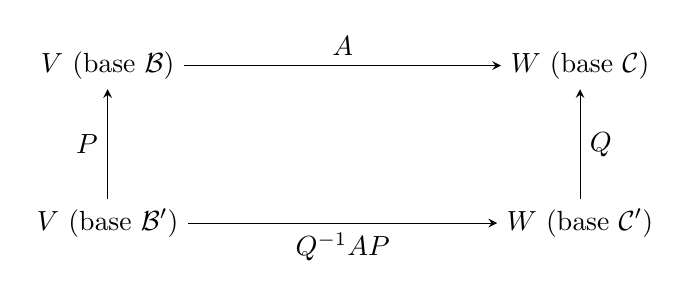
\begin{tikzpicture}[>=stealth, scale=1]
    \node (V1) at (0, 2) {$V$ (base $\mathcal{B}$)};
    \node (W1) at (6, 2) {$W$ (base $\mathcal{C}$)};
    \node (V2) at (0, 0) {$V$ (base $\mathcal{B}'$)};
    \node (W2) at (6, 0) {$W$ (base $\mathcal{C}'$)};

    \draw[->] (V1) -- node[above] {$A$} (W1);
    \draw[->] (V2) -- node[below] {$Q^{-1}AP$} (W2);
    \draw[->] (V2) -- node[left] {$P$} (V1);
    \draw[->] (W2) -- node[right] {$Q$} (W1);
\end{tikzpicture}
\caption{Diagramma commutativo del cambio di base.}
\label{fig:cambio-base}
\end{figure}

\begin{notebox}[Riepilogo del capitolo]
In questo capitolo abbiamo studiato:
\begin{itemize}
    \item La definizione di \textbf{applicazione lineare} e le sue proprietà.
    \item \textbf{Nucleo} e \textbf{immagine} come sottospazi e criteri di iniettività/suriettività.
    \item Il \textbf{teorema della dimensione}: nullità $+$ rango $=$ dimensione del dominio.
    \item La \textbf{matrice associata} come ponte tra applicazioni e matrici.
    \item Il \textbf{cambio di base} e la nozione di matrici simili.
\end{itemize}
\end{notebox}
